\documentclass[12pt,letterpaper]{article}
\usepackage[utf8]{inputenc}
\usepackage[spanish, mexico]{babel}
\usepackage{amsmath}
\usepackage{amsfonts}
\usepackage{amssymb}
\usepackage{amsmath}
\usepackage[lmargin=3cm,rmargin=3cm,tmargin=3cm,bmargin=3cm]{geometry}

\usepackage{hyperref}
\usepackage{graphicx}
\usepackage{float}
\begin{document}

\title{Actividad 8: Iniciandose en Computo Simbolico con Maxima}
\author{Luisa Fernanda Orci Fernandez.}
\date{01 de Abril del 2016}

\maketitle


\section*{Descripción de la actividad}

Para esta actividad se nos pidió leer y explorar el manual $Multivariable$ $Calculus$ $with$ $Maxima$\cite{2}.  \\
 
Maxima es un sistema de álgebra computcional, se especializa en operaciones simbólicas. \cite{1} En Maxima se pueden realizar expansiones de series de Taylor, transformadas de Laplace, también puede resolver matrices, sistemas de ecuaciones líneales, ecuaciones diferenciales, entre otros. \\
Para saber utilizar Maxima fue necesario hacer los ejercicios que venían propuestos en el manual, solo que le modificamos los colores y las funciones. \\

A continuación se muestran los resultados obtenidos.

\section{Geometría en tres dimensiones}

\subsection{Vectores y álgebra líneal}
En esta sección aprendemos a realizar operaciones con vectores; desde como es la notación de
 
Maxima es un sistema de álgebra un vector en Maxima, hasta como operarlos entre si, ya sea sumandolos, multiplicandolos, calculando el producto punto o el producto cruz. A continuación se muestran los resultados obtenidos:

\begin{verbatim}
(%i1) a: [3, 6, 8];
(%o1)                              [3, 6, 8]
(%i2) b: [9, 10, 15];
(%o2)                             [9, 10, 15]
(%i3) 3*a;
(%o3)                             [9, 18, 24]
(%i4) b + a;
(%o4)                            [12, 16, 23]
(%i5)  a.b;
(%o5)                                 207
(%i6) load(vect);
(%o6)           /usr/share/maxima/5.21.1/share/vector/vect.mac
(%i7) a~b;
(%o7)                       [3, 6, 8] ~ [9, 10, 15]
(%i8) express(a~b);
(%o8)                           [10, 27, - 24]
(%i9) 
\end{verbatim}


\subsection{Líneas, planos y superficies cuadráticas}

Aquí se muestra como utilizar el comando $draw3d$, que es para gráficar superficies y el comando $palette$ que es para modificar los colores. A continuación se muestra como utilizar Maxima para graficar un plano, así como un hiperboloide. 

Plano: 

\begin{verbatim}
(%i1) plane1: 4*x + 3*y + 6*z = 0;
(%o1)                         6 z + 3 y + 4 x = 0
(%i2) load(draw);
(%o2)            /usr/share/maxima/5.21.1/share/draw/draw.lisp
(%i3) draw3d(enhanced3d=true,implicit(plane1, x,-4,4, y,-3,3, z,-7,7),palette=[2,5,15]);
(%o3)                          [gr3d(implicit)]
\end{verbatim}

\begin{center}
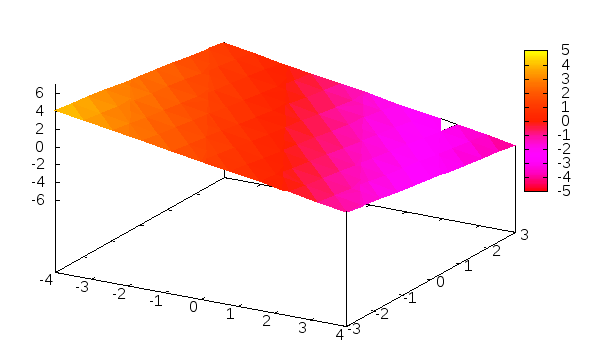
\includegraphics[scale=0.6]{plano1.png}
\end{center}

Hiperboloide: 
\begin{verbatim}
                                 2    2    2
(%o1)                         - z  + y  + x  = 1
(%i2) load(draw);
(%o2)            /usr/share/maxima/5.21.1/share/draw/draw.lisp
(%i3) draw3d(enhanced3d=true, implicit(hyperboloid, x,-2,2, y,-2,2, z,-1.5,1.5), palette=[2,5,15]);
(%o3)                          [gr3d(implicit)]
\end{verbatim}

\begin{center}
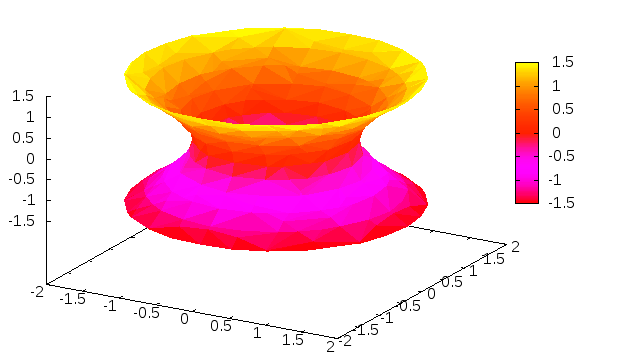
\includegraphics[scale=0.6]{hiperboloide.png}
\end{center}



\subsection{Funciones vectoriales evaluadas}
Aquí propusimos una función, se evaluó en un  punto, calculamos su límite y su derivada y se graficó, todo esto fue posible gracias a que se siguió el manual de Maxima. 

\begin{verbatim}
(%i1) r(t) := [t, cos(t), sin(t)];
(%o1)                     r(t) := [t, cos(t), sin(t)]
(%i2) r(2);
(%o2)                         [2, cos(2), sin(2)]
(%i3) float(r(2));
(%o3)             [2.0, - 0.41614683654714, 0.90929742682568]
(%i4) load(draw);
(%o4)            /usr/share/maxima/5.21.1/share/draw/draw.lisp
(%i5)  draw3d(parametric(cos(t), -cos(t), sin(t), t, -4, 4));
(%o5)                         [gr3d(parametric)]

(%i6)limit(r(t), t, 2);
(%o6)                         [2, cos(2), sin(2)]
(%i7) float(limit(r(t), t, 2));
(%o7)             [2.0, - 0.41614683654714, 0.90929742682568]
(%i8) limit(r(t), t, 2, plus);
(%o8)                         [2, cos(2), sin(2)]
(%i9) limit(r(t), t, 3, minus);
(%o9)                         [3, cos(3), sin(3)]
(%i10) diff(r(t), t);
(%o10)                       [1, - sin(t), cos(t)]
(%i11) 
\end{verbatim}

\begin{center}
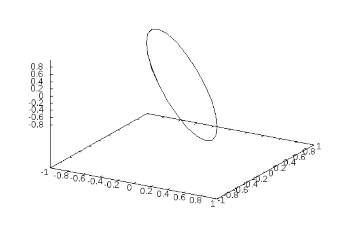
\includegraphics[scale=0.6]{funcion1.png}
\end{center}

\subsection{Longitud de arco y curvatura}
En esta sección se realizó un ejemplo de curvatura que fue propuesto por el manual de Maxima, y se utilizó la fórmula de la curvatura. En este ejercicio Maxima se utilizo como herramienta, ya que el software no es capaz de calcular la curvatura, este ejecuta los pasos para poderla calcular, la curvatura se define de la siguiente forma: 
$$ k = \frac{||r'(t)\times r''(t)||}{||r'(t)^3||} $$

Utilizando esta definición, pudimos obtener los componentes para calcularla:

\begin{verbatim}
(%i1) f(t) := [t, cos(t), sin(t)];
(%o1)                     f(t) := [t, cos(t), sin(t)]
(%i2) fp(t) := [1, -sin(t), cos(t)];
(%o2)                   fp(t) := [1, - sin(t), cos(t)]
(%i3) Tp(t) := [0, -cos(t), sin(t)]/sqrt(2);
                                 [0, - cos(t), sin(t)]
(%o3)                   Tp(t) := ---------------------
                                        sqrt(2)
(%i4) sqrt(Tp(t).Tp(t))/sqrt(rp(t).rp(t));
                                    2         2
                                 sin (t)   cos (t)
                            sqrt(------- + -------)
                                    2         2
(%o4)                       -----------------------
                                          <2>
                                sqrt(rp(t)   )
(%i5) trigsimp(sqrt(Tp(t).Tp(t))/sqrt(rp(t).rp(t)));
                                      1
(%o5)                       ----------------------
                                              <2>
                            sqrt(2) sqrt(rp(t)   )
(%i6) define(kappa(t), sqrt(Tp(t).Tp(t))/sqrt(rp(t).rp(t)));
                                          2         2
                                       sin (t)   cos (t)
                                  sqrt(------- + -------)
                                          2         2
(%o6)                 kappa(t) := -----------------------
                                                <2>
                                      sqrt(rp(t)   )
(%i7) integrate(f(t), t);
                              2
                             t
(%o7)                       [--, sin(t), - cos(t)]
                             2
(%i8) g(t):= [2*t, 3*sin(t), 3*cos(t)];
(%o8)                  g(t) := [2 t, 3 sin(t), 3 cos(t)]
(%i9) define(gp(t), diff(g(t), t));
(%o9)                 gp(t) := [2, 3 cos(t), - 3 sin(t)]
(%i10) integrate(trigsimp(sqrt(gp(t).gp(t))), t, 0, 2*%pi);
(%o10)                          2 sqrt(13) %pi
(%o11)                         22.65434679827795
(%i12) 
\end{verbatim}

\section{Funciones de varias variables}

\subsection{Derivadas parciales}
Se propuso una función  de varias variables y calculamos su derivada parcial con el comando utilizado para calcular una derivada total, la diferencia fue que ahora se le especificó a Maxima con respecto a que variable se quería operar.

\begin{verbatim}
(%i1) diff(f(x,y), x);
                                 d
(%o1)                            -- (f(x, y))
                                 dx
(%i2) diff(diff(f(x,y), x), x);
                                  2
                                 d
(%o2)                            --- (f(x, y))
                                   2
                                 dx
(%i3) diff(diff(f(x,y), x), y);
                                  2
                                 d
(%o3)                           ----- (f(x, y))
                                dx dy
(%i4) G: x^6 * y^5 ;
                                      6  5
(%o4)                                x  y
(%i5) diff(G, x, 1, y, 2, x, 3);
                                        2  3
(%o5)                             7200 x  y
(%i6) 
\end{verbatim}

\subsection{Aproximación líneal}
Aquí se utilizó un polinomio de Taylor para aproximar una función. Maxima facilitó las coas, ya que cuenta con un comando para realizar este tipo de aproximaciones.

\begin{verbatim}
(%i1) f(x, y) := exp(x^2) * sin(y);
                                           2
(%o1)                      f(x, y) := exp(x ) sin(y)
(%i2) taylor(f(x,y), [x,y], [1,2], 1);
(%o2)/T/ sin(2) %e + (2 sin(2) %e (x - 1) + cos(2) %e (y - 2)) + . . .
(%i3) diff(f(x,y));
                     2                        2
                    x                        x
(%o3)             %e   cos(y) del(y) + 2 x %e   sin(y) del(x)
(%i4) 
\end{verbatim}

\subsection{Regla de la cadena}
Aquí volvimos a utilizar la función anterior, pero esta vez la diferenciamos por la regla de la cadena en Maxima. Fue necesario parametrizar esta función y diferenciarla con respecto a cada una de las variables nuevas: 

\begin{verbatim}
(%i1) f(x,y) := exp(x^2) * sin(y);
                                           2
(%o1)                      f(x, y) := exp(x ) sin(y)
(%i2) [x, y] : [s^2 * t, s*t^2];
                                   2       2
(%o2)                            [s  t, s t ]
(%i3) diff(f(x,y), s);
                          4  2                   4  2
                  3  2   s  t         2     2   s  t         2
(%o3)          4 s  t  %e      sin(s t ) + t  %e      cos(s t )
(%i4) diff(f(x,y), t);
                        4  2                      4  2
                 4     s  t         2            s  t         2
(%o4)         2 s  t %e      sin(s t ) + 2 s t %e      cos(s t )
(%i5) diff(f(x,y), x);

                                                 2
diff: second argument must be a variable; found s  t
 -- an error. To debug this try: debugmode(true);
(%i6) diff(f(u,v), u);
                                       2
                                      u
(%o6)                           2 u %e   sin(v)
(%i7) kill(x,y);
(%o7)                                done
(%i8) diff(f(x,y), x);
                                       2
                                      x
(%o8)                           2 x %e   sin(y)
(%i9) 
\end{verbatim}

\subsection{Derivada direccional y gradiente}
Se propuso una función, la cual se convirtió en función vectorial para así poder calcular su gradiente con Maxima, ya que cuenta con un comando especifico para este calculo. Una vez que se obtiene el gradiente, este se evalua en un punto y se calcula la derivada direccional con la una formula previamente aprendida en el curso de Cálculo III:

\begin{verbatim}
(%i1) f(x,y) := exp(x^2) * cos(y);
                                           2
(%o1)                      f(x, y) := exp(x ) cos(y)
(%i2) load(vect);
(%o2)           /usr/share/maxima/5.21.1/share/vector/vect.mac
(%i3) scalefactors([x,y]);
(%o3)                                done
(%i4) gdf: grad(f(x,y));
                                       2
                                      x
(%o4)                         grad (%e   cos(y))
(%i5) ev(express(gdf), diff);
                               2              2
                              x              x
(%o5)                  [2 x %e   cos(y), - %e   sin(y)]
(%i6) define(gdf(x,y), ev(express(gdf), diff));
                                      2              2
                                     x              x
(%o6)            gdf(x, y) := [2 x %e   cos(y), - %e   sin(y)]
(%i7) v: [3, 4];
(%o7)                               [3, 4]
(%i8) (gdf(1,2).v)/sqrt(v.v);
                           6 %e cos(2) - 4 %e sin(2)
(%o8)                      -------------------------
                                       5
(%i9) ev((gdf(1,2).v)/sqrt(v.v), diff);
                           6 %e cos(2) - 4 %e sin(2)
(%o9)                      -------------------------
                                       5
(%i10) float(ev((gdf(1,2).v)/sqrt(v.v), diff));
(%o10)                        - 3.334826598112032
(%i11) sqrt(gdf(1,2).gdf(1,2));
                              2    2          2    2
(%o11)                 sqrt(%e  sin (2) + 4 %e  cos (2))
(%i12) float(ev((gdf(1,2).v)/sqrt(v.v), diff));
(%o12)                        - 3.334826598112032
(%i13) 
\end{verbatim}

\subsection{Optimización y Extremos locales}
De nuevo se propuso una función y se graficó y se siguió un procedimiento para optimizar propuesto por el manual, se utilizaron las derivadas parciales y una matriz a la cual se le calculó el determinante, todo esto para calcular el punto crítico de una función:

\begin{verbatim}
(%i1) f(x,y) := 3*x^2 + 2*y^3 - 8*x*y;
                                    2      3
(%o1)                 f(x, y) := 3 x  + 2 y  + (- 8) x y
(%i2) load(draw);
(%o2)            /usr/share/maxima/5.21.1/share/draw/draw.lisp
(%i3) draw3d(enhanced3d = true, explicit(f(x,y), x, -2,2, y,-2,2), palette=[2,5,15]);
(%o3)                          [gr3d(explicit)]
\end{verbatim}

\begin{center}
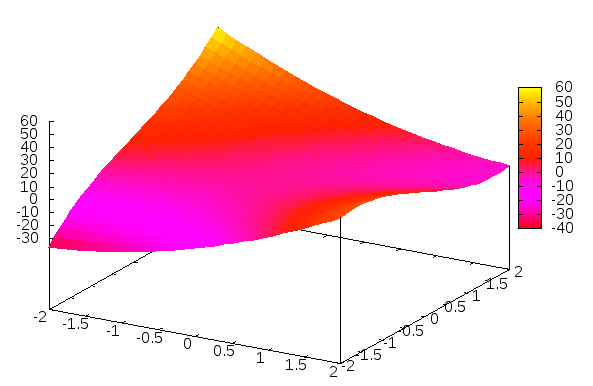
\includegraphics[scale=0.6]{cosa1.png}
\end{center}

\begin{verbatim}
(%i4)draw3d(explicit(f(x,y), x,-2,2, y,-2,2), contour=map, palette=[2,5,15]);
(%o4)                          [gr3d(explicit)]
\end{verbatim}
\begin{center}
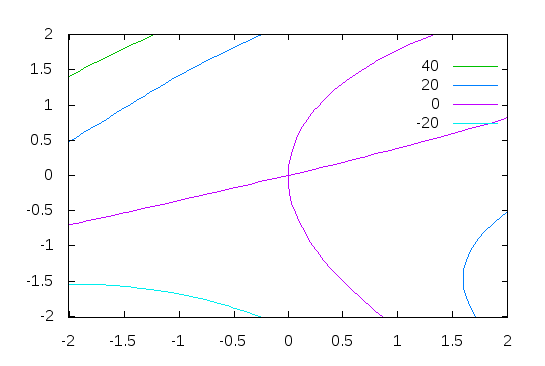
\includegraphics[scale=0.6]{cosa2.png}
\end{center}

\begin{verbatim}
(%i5) fx: diff(f(x,y), x);
(%o5)                              6 x - 8 y
(%i6) fy : diff(f(x,y), y);
                                     2
(%o6)                             6 y  - 8 x
(%i7) solve([fx, fy], [x,y]);
                            64      16
(%o7)                 [[x = --, y = --], [x = 0, y = 0]]
                            27      9
(%i8) H: hessian(f(x,y), [x,y]);
                                 [  6   - 8  ]
(%o8)                            [           ]
                                 [ - 8  12 y ]
(%i9) determinant(H);
(%o9)                              72 y - 64
(%i10) subst([x = -1, y=-1], diff(fx, x));
(%o10)                                 6
(%i11) subst([x = -1, y = -1], determinant(H));
(%o11)                               - 136
(%i12) f(-1, 1);
(%o12)                                13
(%i13) 
\end{verbatim}

\subsection{Multiplicador de Lagrange}
En esta sección se calcularon los valores extremos de una superficie que estaba limitada por otra y para lograr esto, se propusieron dos funciones, estas se diferenciaron y se resolvió el sistema de ecuaciones diferencles para poder encontrar los valores extremos y al final se evaluó esta función en esos puntos para poder encontrar el máxio y mínimo:

\begin{verbatim}
%i1) f(x,y) := 4*x^2 + y^2;
                                           2    2
(%o1)                        f(x, y) := 4 x  + y
(%i2)  g: x^2 + y^2;
                                     2    2
(%o2)                               y  + x
(%i3) eq1: diff(f(x,y), x) = h*diff(g,x);
(%o3)                             8 x = 2 h x
(%i4) eq2: diff(f(x,y), y) = h*diff(g,y);
(%o4)                             2 y = 2 h y
(%i5) eq3: g=1;
                                   2    2
(%o5)                             y  + x  = 1
(%i6) solve([eq1, eq2, eq3], [x, y, h]);
(%o6) [[x = 1, y = 0, h = 4], [x = - 1, y = 0, h = 4], 
                                [x = 0, y = - 1, h = 1], [x = 0, y = 1, h = 1]]
(%i7) [f(1,0), f(-1,0), f(0,-1), f(0,1)];
(%o7)                            [4, 4, 1, 1]
(%i8) 
\end{verbatim}

\section{Integración múltiple}

\subsection{Integrales dobles}
Aquí le proporcionamos una función a Maxima y doblando el comando predeterminado para integrar, Maxima calculó la doble integral de esta función y quedó lo siguiente:

\begin{verbatim}
(%i1) f(x,y) := x^4 - 4*x*y;
                                         4
(%o1)                        f(x, y) := x  - 4 x y
(%i2) integrate(integrate(f(x,y), y), x);
                                  5
                                 x  y    2  2
(%o2)                            ---- - x  y
                                  5
(%i3) integrate(integrate(f(x,y), y, x^1/2, 2-x), x, 0, 1);
                                       187
(%o3)                                - ---
                                       120
(%i4) 
\end{verbatim}

\subsection{Integración en coordenadas polares}
En cursos como Cálculo III y Cálculo IV, nos hemos encontrado con funciones de dos variables, las cuales podemos integrar mediante la parametrización en coordenadas polares de ellas, a veces esto puede resultar un poco tedioso, pero con Maxima resultó ser muy sencillo, y fue de la siguiente manera: 

\begin{verbatim}
(%i1) f(x,y) := x^2 + y^2;
                                          2    2
(%o1)                         f(x, y) := x  + y
(%i2) [x,y]: [r*cos(theta), r*sin(theta)];
(%o2)                    [r cos(theta), r sin(theta)]
(%i3) integrate(integrate(f(x,y)*r, r, 0, 2*cos(theta)), theta, -%pi/2, %pi/2);
                                     3 %pi
(%o3)                                -----
                                       2
(%i4) 
\end{verbatim}

\subsection{Integrales triples}
Esta sección es casi el ejemplo ideal de como Maxima es una gran herramienta matemática, ya que reduce el integrar una integral triple a un "solo renglón" y puede ser de gran ayuda en un curso de Cálculo III o Cálculo IV. A partir del manual, así quedó el ejemplo de resolver una integral triple con Maxima:

\begin{verbatim}
(%i1) integrate(integrate(integrate(x^3*y*z,z,0,x+y), y,0,-x), x,0,1);
                                       1
(%o1)                                 ---
                                      192
(%i2) 
\end{verbatim}

\subsection{Integrales en Coordenadas esféricas y cilíndricas}
Esta sección es muy parecida a la de integración en coordenadas polares, la diferencia es que se utiliza una parametrización distinta, pero la idea es la misma, y una vez mas, Maxima nos ayudó a realizar esta integración de una forma rápida y sin problemas;\\

Coordenadas cilíndricas:

\begin{verbatim}
(%i1) f(x,y,z) := (y+x)*z;
(%o1)                       f(x, y, z) := (y + x) z
(%i2) [x,y,z] : [r*cos(theta), r*sin(theta), z];
(%o2)                   [r cos(theta), r sin(theta), z]
(%i3) integrate(integrate(integrate(f(x,y,z)*r, z,0,3), r,0,2), theta,0,%pi);
(%o3)                                 24
(%i4) 
\end{verbatim}

Coordenadas esféricas:

\begin{verbatim}
(%i1) f(x,y,z) := x*z;
(%o1)                          f(x, y, z) := x z
(%i2) [x,y,z] : [rho*sin(phi)*cos(theta), rho*sin(phi)*sin(theta), rho*cos(theta)];
(%o2) [sin(phi) rho cos(theta), sin(phi) rho sin(theta), rho cos(theta)]
(%i3) integrate(integrate(integrate(f(x,y,z)*rho^2*sin(phi),rho,0,1),theta,0,%pi),phi,0,%pi/2);
                                        2
                                     %pi
(%o3)                                ----
                                      40
(%i4) 
\end{verbatim}


\subsection{Cambio de variable}

Aquí utilizamos el teorema de integración de cambio de variable, visto previamente en el curso de Cálculo IV: 
$$ \int\int_R f(x, y)dxdy = \int\int_s f(g(u, v), h(u, v)) \begin{vmatrix}
d(x, y) \\ d(u, v)
\end{vmatrix}dudv $$
El código quedó así:

\begin{verbatim}
(%i1) f(x,y) := x+y;
(%o1)                          f(x, y) := x + y
(%i2) [x,y]: [u^3 - v^4, 5*u*v];
                                 3    4
(%o2)                          [u  - v , 5 u v]
(%i3) J: jacobian([x,y], [u,v]);
                               [    2       3 ]
(%o3)                          [ 3 u   - 4 v  ]
                               [              ]
                               [ 5 v    5 u   ]
(%i4) J: determinant(J);
                                     4       3
(%o4)                            20 v  + 15 u
(%i5) integrate(integrate(f(x,y)*J, u,1,2), v,3,4);
                                    113349305
(%o5)                             - ---------
                                       252
(%i6) 
\end{verbatim}


\section{Cálculo vectorial}

\subsection{Campo vectorial}
Aquí tuvimos que graficar campos vectoriales, para lograr esto partimos de una función modificada mediante algunos comandos de Maxima y así se puede graficar como campo vectorial: 

\begin{verbatim}
(%i1) load(draw);
(%o1)            /usr/share/maxima/5.21.1/share/draw/draw.lisp
(%i2) F(x,y):=[cos(y), x];
(%o2)                       F(x, y) := [cos(y), x]
(%i3) coord:setify(makelist(k,k,-6,6));
(%o3)         {- 6, - 5, - 4, - 3, - 2, - 1, 0, 1, 2, 3, 4, 5, 6}
(%i4) points2d:listify(cartesian_product(coord, coord));
(%o4) [[- 6, - 6], [- 6, - 5], [- 6, - 4], [- 6, - 3], [- 6, - 2], [- 6, - 1], 
[- 6, 0], [- 6, 1], [- 6, 2], [- 6, 3], [- 6, 4], [- 6, 5], [- 6, 6], 
[- 5, - 6], [- 5, - 5], [- 5, - 4], [- 5, - 3], [- 5, - 2], [- 5, - 1], 
[- 5, 0], [- 5, 1], [- 5, 2], [- 5, 3], [- 5, 4], [- 5, 5], [- 5, 6], 
[- 4, - 6], [- 4, - 5], [- 4, - 4], [- 4, - 3], [- 4, - 2], [- 4, - 1], 
[- 4, 0], [- 4, 1], [- 4, 2], [- 4, 3], [- 4, 4], [- 4, 5], [- 4, 6], 
[- 3, - 6], [- 3, - 5], [- 3, - 4], [- 3, - 3], [- 3, - 2], [- 3, - 1], 
[- 3, 0], [- 3, 1], [- 3, 2], [- 3, 3], [- 3, 4], [- 3, 5], [- 3, 6], 
[- 2, - 6], [- 2, - 5], [- 2, - 4], [- 2, - 3], [- 2, - 2], [- 2, - 1], 
[- 2, 0], [- 2, 1], [- 2, 2], [- 2, 3], [- 2, 4], [- 2, 5], [- 2, 6], 
[- 1, - 6], [- 1, - 5], [- 1, - 4], [- 1, - 3], [- 1, - 2], [- 1, - 1], 
[- 1, 0], [- 1, 1], [- 1, 2], [- 1, 3], [- 1, 4], [- 1, 5], [- 1, 6], 
[0, - 6], [0, - 5], [0, - 4], [0, - 3], [0, - 2], [0, - 1], [0, 0], [0, 1], 
[0, 2], [0, 3], [0, 4], [0, 5], [0, 6], [1, - 6], [1, - 5], [1, - 4], 
[1, - 3], [1, - 2], [1, - 1], [1, 0], [1, 1], [1, 2], [1, 3], [1, 4], [1, 5], 
[1, 6], [2, - 6], [2, - 5], [2, - 4], [2, - 3], [2, - 2], [2, - 1], [2, 0], 
[2, 1], [2, 2], [2, 3], [2, 4], [2, 5], [2, 6], [3, - 6], [3, - 5], [3, - 4], 
[3, - 3], [3, - 2], [3, - 1], [3, 0], [3, 1], [3, 2], [3, 3], [3, 4], [3, 5], 
[3, 6], [4, - 6], [4, - 5], [4, - 4], [4, - 3], [4, - 2], [4, - 1], [4, 0], 
[4, 1], [4, 2], [4, 3], [4, 4], [4, 5], [4, 6], [5, - 6], [5, - 5], [5, - 4], 
[5, - 3], [5, - 2], [5, - 1], [5, 0], [5, 1], [5, 2], [5, 3], [5, 4], [5, 5], 
[5, 6], [6, - 6], [6, - 5], [6, - 4], [6, - 3], [6, - 2], [6, - 1], [6, 0], 
[6, 1], [6, 2], [6, 3], [6, 4], [6, 5], [6, 6]]
(%i5) vf2d(x,y):=vector([x,y], [cos(y), x]/6);
                                                [cos(y), x]
(%o5)              vf2d(x, y) := vector([x, y], -----------)
                                                     6
(%i6) vect2:makelist(vf2d(k[1],k[2]),k,points2d);
                           cos(6)                             cos(5)
(%o6) [vector([- 6, - 6], [------, - 1]), vector([- 6, - 5], [------, - 1]), 
                             6                                  6
                    cos(4)                             cos(3)
vector([- 6, - 4], [------, - 1]), vector([- 6, - 3], [------, - 1]), 
                      6                                  6
                    cos(2)                             cos(1)
vector([- 6, - 2], [------, - 1]), vector([- 6, - 1], [------, - 1]), 
                      6                                  6
                  1                           cos(1)
vector([- 6, 0], [-, - 1]), vector([- 6, 1], [------, - 1]), 
                  6                             6
                  cos(2)                           cos(3)
vector([- 6, 2], [------, - 1]), vector([- 6, 3], [------, - 1]), 
                    6                                6
                  cos(4)                           cos(5)
vector([- 6, 4], [------, - 1]), vector([- 6, 5], [------, - 1]), 
                    6                                6
                  cos(6)                             cos(6)    5
vector([- 6, 6], [------, - 1]), vector([- 5, - 6], [------, - -]), 
                    6                                  6       6
                    cos(5)    5                        cos(4)    5
vector([- 5, - 5], [------, - -]), vector([- 5, - 4], [------, - -]), 
                      6       6                          6       6
                    cos(3)    5                        cos(2)    5
vector([- 5, - 3], [------, - -]), vector([- 5, - 2], [------, - -]), 
                      6       6                          6       6
                    cos(1)    5                      1    5
vector([- 5, - 1], [------, - -]), vector([- 5, 0], [-, - -]), 
                      6       6                      6    6
                  cos(1)    5                      cos(2)    5
vector([- 5, 1], [------, - -]), vector([- 5, 2], [------, - -]), 
                    6       6                        6       6
                  cos(3)    5                      cos(4)    5
vector([- 5, 3], [------, - -]), vector([- 5, 4], [------, - -]), 
                    6       6                        6       6
                  cos(5)    5                      cos(6)    5
vector([- 5, 5], [------, - -]), vector([- 5, 6], [------, - -]), 
                    6       6                        6       6
                    cos(6)    2                        cos(5)    2
vector([- 4, - 6], [------, - -]), vector([- 4, - 5], [------, - -]), 
                      6       3                          6       3
                    cos(4)    2                        cos(3)    2
vector([- 4, - 4], [------, - -]), vector([- 4, - 3], [------, - -]), 
                      6       3                          6       3
                    cos(2)    2                        cos(1)    2
vector([- 4, - 2], [------, - -]), vector([- 4, - 1], [------, - -]), 
                      6       3                          6       3
                  1    2                      cos(1)    2
vector([- 4, 0], [-, - -]), vector([- 4, 1], [------, - -]), 
                  6    3                        6       3
                  cos(2)    2                      cos(3)    2
vector([- 4, 2], [------, - -]), vector([- 4, 3], [------, - -]), 
                    6       3                        6       3
                  cos(4)    2                      cos(5)    2
vector([- 4, 4], [------, - -]), vector([- 4, 5], [------, - -]), 
                    6       3                        6       3
                  cos(6)    2                        cos(6)    1
vector([- 4, 6], [------, - -]), vector([- 3, - 6], [------, - -]), 
                    6       3                          6       2
                    cos(5)    1                        cos(4)    1
vector([- 3, - 5], [------, - -]), vector([- 3, - 4], [------, - -]), 
                      6       2                          6       2
                    cos(3)    1                        cos(2)    1
vector([- 3, - 3], [------, - -]), vector([- 3, - 2], [------, - -]), 
                      6       2                          6       2
                    cos(1)    1                      1    1
vector([- 3, - 1], [------, - -]), vector([- 3, 0], [-, - -]), 
                      6       2                      6    2
                  cos(1)    1                      cos(2)    1
vector([- 3, 1], [------, - -]), vector([- 3, 2], [------, - -]), 
                    6       2                        6       2
                  cos(3)    1                      cos(4)    1
vector([- 3, 3], [------, - -]), vector([- 3, 4], [------, - -]), 
                    6       2                        6       2
                  cos(5)    1                      cos(6)    1
vector([- 3, 5], [------, - -]), vector([- 3, 6], [------, - -]), 
                    6       2                        6       2
                    cos(6)    1                        cos(5)    1
vector([- 2, - 6], [------, - -]), vector([- 2, - 5], [------, - -]), 
                      6       3                          6       3
                    cos(4)    1                        cos(3)    1
vector([- 2, - 4], [------, - -]), vector([- 2, - 3], [------, - -]), 
                      6       3                          6       3
                    cos(2)    1                        cos(1)    1
vector([- 2, - 2], [------, - -]), vector([- 2, - 1], [------, - -]), 
                      6       3                          6       3
                  1    1                      cos(1)    1
vector([- 2, 0], [-, - -]), vector([- 2, 1], [------, - -]), 
                  6    3                        6       3
                  cos(2)    1                      cos(3)    1
vector([- 2, 2], [------, - -]), vector([- 2, 3], [------, - -]), 
                    6       3                        6       3
                  cos(4)    1                      cos(5)    1
vector([- 2, 4], [------, - -]), vector([- 2, 5], [------, - -]), 
                    6       3                        6       3
                  cos(6)    1                        cos(6)    1
vector([- 2, 6], [------, - -]), vector([- 1, - 6], [------, - -]), 
                    6       3                          6       6
                    cos(5)    1                        cos(4)    1
vector([- 1, - 5], [------, - -]), vector([- 1, - 4], [------, - -]), 
                      6       6                          6       6
                    cos(3)    1                        cos(2)    1
vector([- 1, - 3], [------, - -]), vector([- 1, - 2], [------, - -]), 
                      6       6                          6       6
                    cos(1)    1                      1    1
vector([- 1, - 1], [------, - -]), vector([- 1, 0], [-, - -]), 
                      6       6                      6    6
                  cos(1)    1                      cos(2)    1
vector([- 1, 1], [------, - -]), vector([- 1, 2], [------, - -]), 
                    6       6                        6       6
                  cos(3)    1                      cos(4)    1
vector([- 1, 3], [------, - -]), vector([- 1, 4], [------, - -]), 
                    6       6                        6       6
                  cos(5)    1                      cos(6)    1
vector([- 1, 5], [------, - -]), vector([- 1, 6], [------, - -]), 
                    6       6                        6       6
                  cos(6)                         cos(5)
vector([0, - 6], [------, 0]), vector([0, - 5], [------, 0]), 
                    6                              6
                  cos(4)                         cos(3)
vector([0, - 4], [------, 0]), vector([0, - 3], [------, 0]), 
                    6                              6
                  cos(2)                         cos(1)
vector([0, - 2], [------, 0]), vector([0, - 1], [------, 0]), 
                    6                              6
                1                       cos(1)
vector([0, 0], [-, 0]), vector([0, 1], [------, 0]), 
                6                         6
                cos(2)                       cos(3)
vector([0, 2], [------, 0]), vector([0, 3], [------, 0]), 
                  6                            6
                cos(4)                       cos(5)
vector([0, 4], [------, 0]), vector([0, 5], [------, 0]), 
                  6                            6
                cos(6)                         cos(6)  1
vector([0, 6], [------, 0]), vector([1, - 6], [------, -]), 
                  6                              6     6
                  cos(5)  1                      cos(4)  1
vector([1, - 5], [------, -]), vector([1, - 4], [------, -]), 
                    6     6                        6     6
                  cos(3)  1                      cos(2)  1
vector([1, - 3], [------, -]), vector([1, - 2], [------, -]), 
                    6     6                        6     6
                  cos(1)  1                    1  1
vector([1, - 1], [------, -]), vector([1, 0], [-, -]), 
                    6     6                    6  6
                cos(1)  1                    cos(2)  1
vector([1, 1], [------, -]), vector([1, 2], [------, -]), 
                  6     6                      6     6
                cos(3)  1                    cos(4)  1
vector([1, 3], [------, -]), vector([1, 4], [------, -]), 
                  6     6                      6     6
                cos(5)  1                    cos(6)  1
vector([1, 5], [------, -]), vector([1, 6], [------, -]), 
                  6     6                      6     6
                  cos(6)  1                      cos(5)  1
vector([2, - 6], [------, -]), vector([2, - 5], [------, -]), 
                    6     3                        6     3
                  cos(4)  1                      cos(3)  1
vector([2, - 4], [------, -]), vector([2, - 3], [------, -]), 
                    6     3                        6     3
                  cos(2)  1                      cos(1)  1
vector([2, - 2], [------, -]), vector([2, - 1], [------, -]), 
                    6     3                        6     3
                1  1                    cos(1)  1
vector([2, 0], [-, -]), vector([2, 1], [------, -]), 
                6  3                      6     3
                cos(2)  1                    cos(3)  1
vector([2, 2], [------, -]), vector([2, 3], [------, -]), 
                  6     3                      6     3
                cos(4)  1                    cos(5)  1
vector([2, 4], [------, -]), vector([2, 5], [------, -]), 
                  6     3                      6     3
                cos(6)  1                      cos(6)  1
vector([2, 6], [------, -]), vector([3, - 6], [------, -]), 
                  6     3                        6     2
                  cos(5)  1                      cos(4)  1
vector([3, - 5], [------, -]), vector([3, - 4], [------, -]), 
                    6     2                        6     2
                  cos(3)  1                      cos(2)  1
vector([3, - 3], [------, -]), vector([3, - 2], [------, -]), 
                    6     2                        6     2
                  cos(1)  1                    1  1
vector([3, - 1], [------, -]), vector([3, 0], [-, -]), 
                    6     2                    6  2
                cos(1)  1                    cos(2)  1
vector([3, 1], [------, -]), vector([3, 2], [------, -]), 
                  6     2                      6     2
                cos(3)  1                    cos(4)  1
vector([3, 3], [------, -]), vector([3, 4], [------, -]), 
                  6     2                      6     2
                cos(5)  1                    cos(6)  1
vector([3, 5], [------, -]), vector([3, 6], [------, -]), 
                  6     2                      6     2
                  cos(6)  2                      cos(5)  2
vector([4, - 6], [------, -]), vector([4, - 5], [------, -]), 
                    6     3                        6     3
                  cos(4)  2                      cos(3)  2
vector([4, - 4], [------, -]), vector([4, - 3], [------, -]), 
                    6     3                        6     3
                  cos(2)  2                      cos(1)  2
vector([4, - 2], [------, -]), vector([4, - 1], [------, -]), 
                    6     3                        6     3
                1  2                    cos(1)  2
vector([4, 0], [-, -]), vector([4, 1], [------, -]), 
                6  3                      6     3
                cos(2)  2                    cos(3)  2
vector([4, 2], [------, -]), vector([4, 3], [------, -]), 
                  6     3                      6     3
                cos(4)  2                    cos(5)  2
vector([4, 4], [------, -]), vector([4, 5], [------, -]), 
                  6     3                      6     3
                cos(6)  2                      cos(6)  5
vector([4, 6], [------, -]), vector([5, - 6], [------, -]), 
                  6     3                        6     6
                  cos(5)  5                      cos(4)  5
vector([5, - 5], [------, -]), vector([5, - 4], [------, -]), 
                    6     6                        6     6
                  cos(3)  5                      cos(2)  5
vector([5, - 3], [------, -]), vector([5, - 2], [------, -]), 
                    6     6                        6     6
                  cos(1)  5                    1  5
vector([5, - 1], [------, -]), vector([5, 0], [-, -]), 
                    6     6                    6  6
                cos(1)  5                    cos(2)  5
vector([5, 1], [------, -]), vector([5, 2], [------, -]), 
                  6     6                      6     6
                cos(3)  5                    cos(4)  5
vector([5, 3], [------, -]), vector([5, 4], [------, -]), 
                  6     6                      6     6
                cos(5)  5                    cos(6)  5
vector([5, 5], [------, -]), vector([5, 6], [------, -]), 
                  6     6                      6     6
                  cos(6)                         cos(5)
vector([6, - 6], [------, 1]), vector([6, - 5], [------, 1]), 
                    6                              6
                  cos(4)                         cos(3)
vector([6, - 4], [------, 1]), vector([6, - 3], [------, 1]), 
                    6                              6
                  cos(2)                         cos(1)
vector([6, - 2], [------, 1]), vector([6, - 1], [------, 1]), 
                    6                              6
                1                       cos(1)
vector([6, 0], [-, 1]), vector([6, 1], [------, 1]), 
                6                         6
                cos(2)                       cos(3)
vector([6, 2], [------, 1]), vector([6, 3], [------, 1]), 
                  6                            6
                cos(4)                       cos(5)
vector([6, 4], [------, 1]), vector([6, 5], [------, 1]), 
                  6                            6
                cos(6)
vector([6, 6], [------, 1])]
                  6
(%i7) apply(draw2d,append([color=magenta],vect2));
(%o7) [gr2d(vector, vector, vector, vector, vector, vector, vector, vector, 
vector, vector, vector, vector, vector, vector, vector, vector, vector, 
vector, vector, vector, vector, vector, vector, vector, vector, vector, 
vector, vector, vector, vector, vector, vector, vector, vector, vector, 
vector, vector, vector, vector, vector, vector, vector, vector, vector, 
vector, vector, vector, vector, vector, vector, vector, vector, vector, 
vector, vector, vector, vector, vector, vector, vector, vector, vector, 
vector, vector, vector, vector, vector, vector, vector, vector, vector, 
vector, vector, vector, vector, vector, vector, vector, vector, vector, 
vector, vector, vector, vector, vector, vector, vector, vector, vector, 
vector, vector, vector, vector, vector, vector, vector, vector, vector, 
vector, vector, vector, vector, vector, vector, vector, vector, vector, 
vector, vector, vector, vector, vector, vector, vector, vector, vector, 
vector, vector, vector, vector, vector, vector, vector, vector, vector, 
vector, vector, vector, vector, vector, vector, vector, vector, vector, 
vector, vector, vector, vector, vector, vector, vector, vector, vector, 
vector, vector, vector, vector, vector, vector, vector, vector, vector, 
vector, vector, vector, vector, vector, vector, vector, vector, vector, 
vector, vector, vector, vector, vector, vector, vector, vector)]
(%i8) 
\end{verbatim}

\subsection{Integrales de línea}
Aquí pudimos ver como resolver integrales de línea con respecto a la longitud de arco: 

\begin{verbatim}
(%i1) f(x,y):= x^2 + y^2;
                                          2    2
(%o1)                         f(x, y) := x  + y
(%i2) [x,y]: [cos(t), sin(2*t)];
(%o2)                         [cos(t), sin(2 t)]
(%i3) rp: diff([x,y], t);
(%o3)                       [- sin(t), 2 cos(2 t)]
(%i4) romberg(f(x,y)*sqrt(rp.rp),t,0,1);
(%o4)                          1.635879048260743
(%i5) 
\end{verbatim}

\subsection{Campos vectoriales conservativos y Potenciales escalares}
Aquí calculamos el rotacional de un campo gradiente para saber si es o no es conservativo:

\begin{verbatim}
(%i1) F(x,y) := [3*x^3 - 6*y^2, 3*y^3-5*x];
                                    3      2     3
(%o1)                F(x, y) := [3 x  - 6 y , 3 y  - 5 x]
(%i2) load(vect);
(%o2)           /usr/share/maxima/5.21.1/share/vector/vect.mac
(%i3) scalefactors([x,y]);
(%o3)                                done
(%i4) curl(F(x,y));
                                 3      2     3
(%o4)                   curl [3 x  - 6 y , 3 y  - 5 x]
(%i5) express(curl(F(x,y)));
                      d      3          d      3      2
(%o5)                 -- (3 y  - 5 x) - -- (3 x  - 6 y )
                      dx                dy
(%i6) ev(express(curl(F(x,y))), diff);
(%o6)                              12 y - 5
(%i7) 
\end{verbatim}




\section*{Conclusiones}
Esta fue una actividad muy larga, pero de gran ayuda para el futuro, ya que fue un tutorial de como utilizar Maxima, que es una gran herramienta matématica.

\begin{thebibliography}{widestlabel}
      \bibitem{1} Wikipedia, \emph{Maxima}, (2016, 01 de Abril).Desde: \url{https://es.wikipedia.org/wiki/Maxima}
      \bibitem{2} gkerns, \emph{Multivariable Calculus with Maxima}, (2016, 01 de Abril).Desde: \url{http://gkerns.people.ysu.edu/maxima/maximaintro/}
\end{thebibliography}


\end{document}